% block_diagram.tex -- top-level block diagram of the direct-mapped cache
% Owner: Member 1. Compiles standalone to PDF; include the PDF in the IEEE
% report with \includegraphics[width=\columnwidth]{figures/block_diagram.pdf}
\documentclass[tikz,border=6pt]{standalone}
\usetikzlibrary{arrows.meta,calc}
\begin{document}
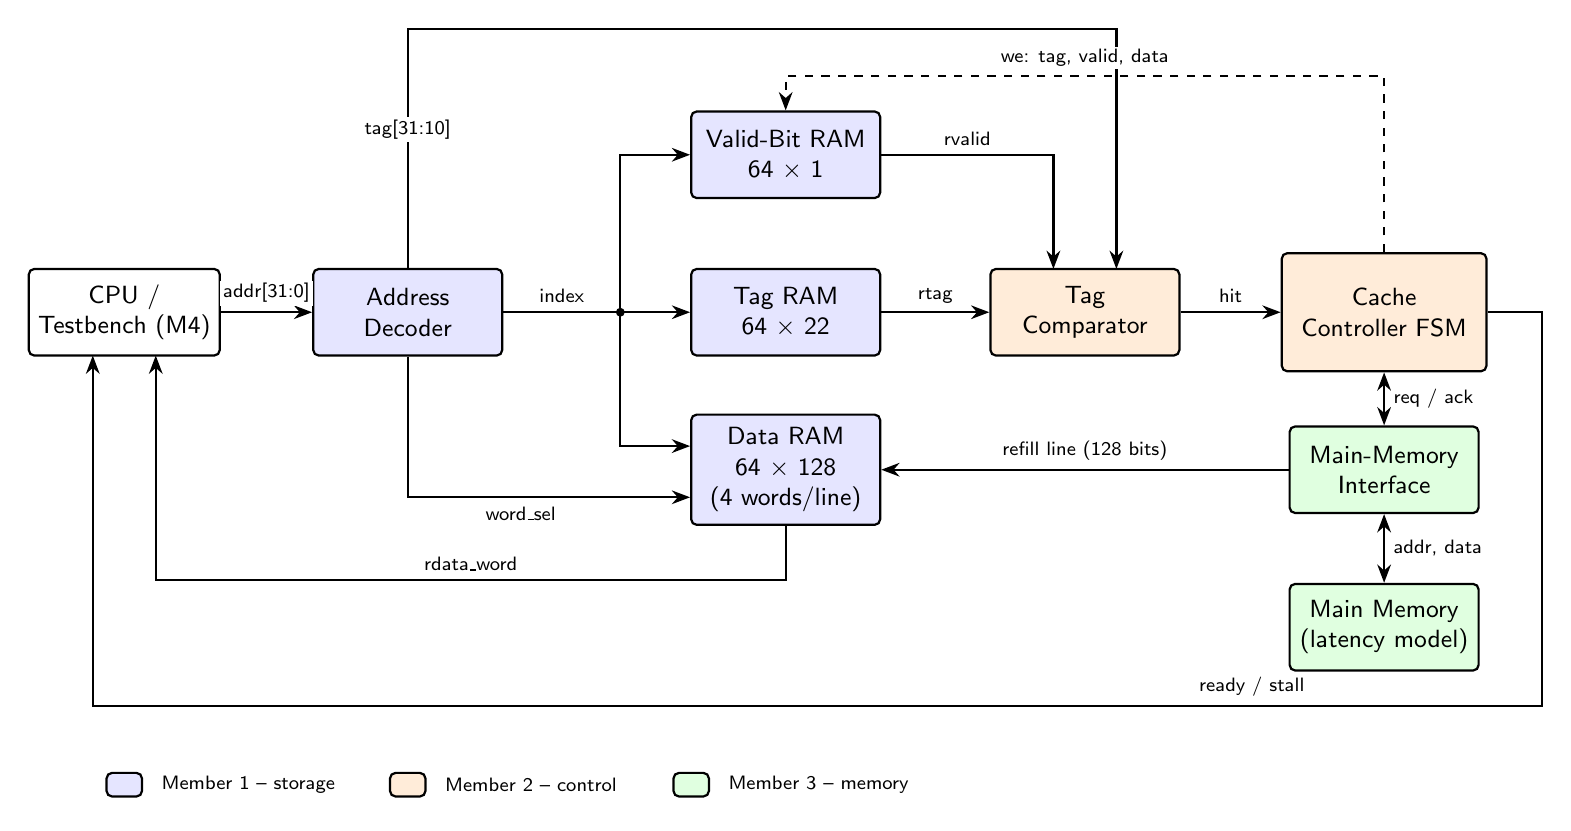
\begin{tikzpicture}[
    >=Stealth, font=\sffamily\small,
    blk/.style={draw, thick, rounded corners=2pt, align=center, minimum height=1.1cm, minimum width=2.4cm, fill=white},
    m1/.style={blk, fill=blue!10},
    m2/.style={blk, fill=orange!15},
    m3/.style={blk, fill=green!12},
    lbl/.style={font=\sffamily\scriptsize, fill=white, inner sep=1pt},
]
% ---------------- blocks ----------------
\node[blk, minimum width=2cm] (cpu)   at (0,0)      {CPU /\\Testbench (M4)};
\node[m1]                     (dec)   at (3.6,0)    {Address\\Decoder};
\node[m1]                     (valid) at (8.4,2.0)  {Valid-Bit RAM\\64 $\times$ 1};
\node[m1]                     (tag)   at (8.4,0)    {Tag RAM\\64 $\times$ 22};
\node[m1, minimum height=1.4cm] (data) at (8.4,-2.0) {Data RAM\\64 $\times$ 128\\(4 words/line)};
\node[m2]                     (cmp)   at (12.2,0)   {Tag\\Comparator};
\node[m2, minimum width=2.6cm, minimum height=1.5cm] (fsm) at (16.0,0) {Cache\\Controller FSM};
\node[m3]                     (mif)   at (16.0,-2.0) {Main-Memory\\Interface};
\node[m3]                     (mem)   at (16.0,-4.0) {Main Memory\\(latency model)};

% ---------------- address path ----------------
\draw[->, thick] (cpu) -- node[lbl, above=2pt]{addr[31:0]} (dec);

\coordinate (bus) at (6.3,0);
\draw[thick] (dec.east) -- node[lbl, above=2pt]{index} (bus);
\draw[->, thick] (bus) |- (valid.west);
\draw[->, thick] (bus) -- (tag.west);
\draw[->, thick] (bus) |- ($(data.west)+(0,0.3)$);
\fill (bus) circle (1.6pt);

\draw[->, thick] (dec.south) |- node[lbl, pos=0.7, below=2pt]{word\_sel} ($(data.west)+(0,-0.35)$);

% tag field goes over the top to the comparator
\draw[->, thick] (dec.north) |- (12.6,3.6) node[lbl, pos=0.25, above=2pt]{tag[31:10]} -- (12.6,0.55);

% ---------------- lookup ----------------
\draw[->, thick] (valid.east) -| node[lbl, pos=0.25, above=2pt]{rvalid} (11.8,0.55);
\draw[->, thick] (tag.east) -- node[lbl, above=2pt]{rtag} (cmp.west);
\draw[->, thick] (cmp) -- node[lbl, above=2pt]{hit} (fsm);

% ---------------- control (FSM -> storage write enables) ----------------
\draw[->, thick, dashed] (fsm.north) |- (8.4,3.0) node[lbl, pos=0.75, above=2pt]{we: tag, valid, data} -- (valid.north);

% ---------------- refill path ----------------
\draw[<->, thick] (fsm) -- node[lbl, right=2pt]{req / ack} (mif);
\draw[<->, thick] (mif) -- node[lbl, right=2pt]{addr, data} (mem);
\draw[->, thick] (mif.west) -- node[lbl, above=2pt]{refill line (128 bits)} (data.east);

% ---------------- back to CPU ----------------
\draw[->, thick] (data.south) |- (0.4,-3.4) node[lbl, pos=0.75, above=2pt]{rdata\_word} -- (0.4,-0.55);
\draw[->, thick] (fsm.east) -- (18.0,0) |- (-0.4,-5.0) node[lbl, pos=0.6, above=2pt]{ready / stall} -- (-0.4,-0.55);

% ---------------- legend ----------------
\begin{scope}[shift={(0,-6.0)}]
  \node[m1, minimum width=0.45cm, minimum height=0.3cm] (l1) at (0,0) {};
  \node[anchor=west, font=\sffamily\scriptsize] at (0.35,0) {Member 1 -- storage};
  \node[m2, minimum width=0.45cm, minimum height=0.3cm] (l2) at (3.6,0) {};
  \node[anchor=west, font=\sffamily\scriptsize] at (3.95,0) {Member 2 -- control};
  \node[m3, minimum width=0.45cm, minimum height=0.3cm] (l3) at (7.2,0) {};
  \node[anchor=west, font=\sffamily\scriptsize] at (7.55,0) {Member 3 -- memory};
\end{scope}
\end{tikzpicture}
\end{document}
